\documentclass{beamer}

\usepackage[utf8]{inputenc}
\usepackage{hyperref}

\usetheme{Berkeley}
\beamertemplatenavigationsymbolsempty
\setbeamertemplate{headline}{}
 
\title{FoodChain-Lab Introduction}
\date{}
 
\begin{document}
\maketitle

\section{FoodChain-Lab Concepts 1}
\begin{frame}
	\begin{itemize}
		\item \textbf{Delivery}: Something sent from A to B at a certain date. A delivery can have preceding and subsequent deliveries (e.g. strawberry-delivery -$>$ strawberry-cake-delivery).
		\item \textbf{Station}: Any food business operator, that sends and/or receives deliveries.
		\item \textbf{Trace}: The path a contamination can take. A station/delivery "B" is on the \textbf{forward trace} of a station/delivery "A", if a contamination at "A" can spread to "B" via the food chain network. If "B" is on the \textbf{forward trace} of "A", then "A" is on the \textbf{backward trace} of "B".
	\end{itemize}
\end{frame}

\section{FoodChain-Lab Concepts 2}
\begin{frame}
	\begin{itemize}
		\item \textbf{Weight}: Weights are assigned to stations/deliveries, that are involved in an outbreak (e.g. a restaurant where customers got sick). Different weights can be used to model differences between involved stations/deliveries (e.g. higher weight = higher likelihood that station is involved)..
		\item \textbf{Cross Contamination}: When it is applied at a station, its incoming deliveries contaminate its outgoing deliveries. When applied on delivery level, the selected incoming deliveries of station contaminate each others subsequent deliveries.
		\item \textbf{Kill Contamination}: When it is applied at a station/delivery, the contamination is killed there. That means it does not spread to subsequent stations/deliveries.
		\item \textbf{Score}: Is computed based on given weights and cross contamination. Should help to estimate the likelihood that a certain station is the origin of the outbreak (higher score = more/higher weighted stations on forward trace).
	\end{itemize}
\end{frame}

\section{FoodChain-Lab Score Computation 1}
\begin{frame}
	\begin{center}
  		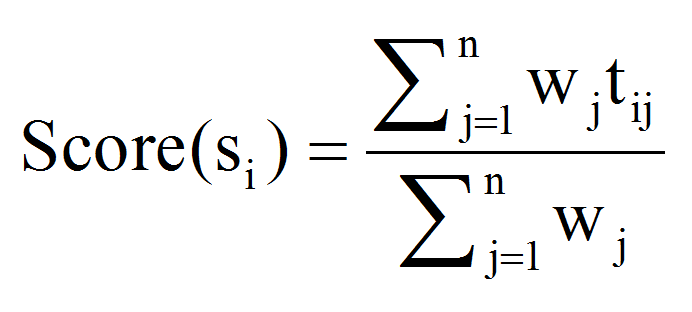
\includegraphics[height=0.3\textheight]{score.png}
	\end{center}
	\begin{itemize}
		\item $s_i$ is the i-th station or delivery
		\item $w_j$ is the weight of the j-th station or delivery
		\item $t_{ij}$ has a value of 1, if there is a trace from $s_i$ to $s_j$ and a value of 0 otherwise
		\item $n$ is the total number of stations and deliveries
	\end{itemize}
\end{frame}

\section{FoodChain-Lab Score Computation 2}
\begin{frame}
	\begin{center}
  		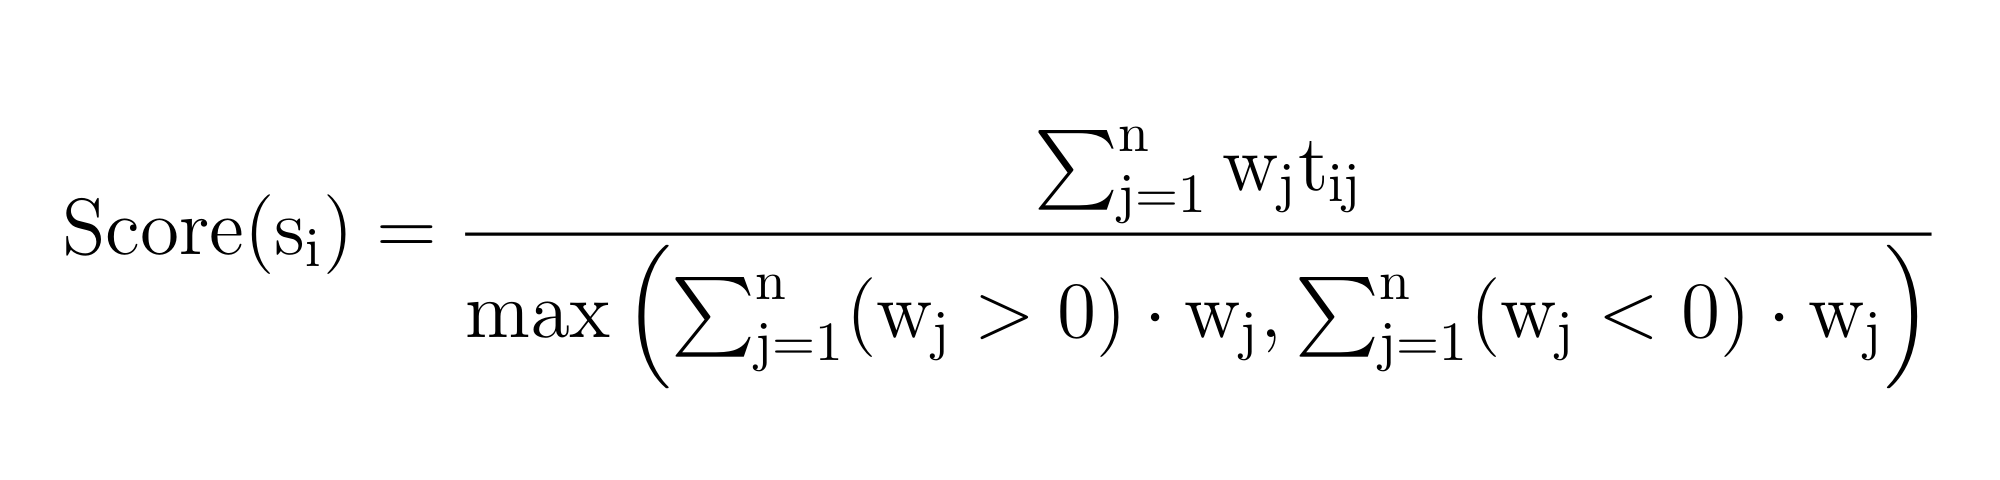
\includegraphics[width=0.9\textwidth]{new_score.png}
	\end{center}
	\begin{itemize}
		\item FoodChain-Lab also allows to assign negative weights to stations/deliveries.
		\item A negative weight should indicate, that a station/delivery is not involved in the outbreak.
		\item When negative weights are used, the score computation changes to this formula.
	\end{itemize}
\end{frame}

\section{Introduction to KNIME}
\begin{frame}
	\begin{itemize}
		\item KNIME is an open source data analytics platform, that allows users to assemble a data pipeline called "workflow".
		\item A workflow is built by dragging nodes from the \textbf{Node Repository} onto the \textbf{Workflow Editor} and connecting them (\url{https://tech.knime.org/workbench}).
		\item Nodes are processing units with input- and/or output ports.
		\item Data is transferred over a connection from an out-port to the in-port of another node.
		\item A comprehensive KNIME quickstart guide can be found at \url{https://tech.knime.org/files/KNIME_quickstart.pdf}.
		\item An introduction video is available at \url{https://www.youtube.com/watch?v=ft7Ksgss3Tc}.
	\end{itemize}
\end{frame}

\section{Available Nodes}
\begin{frame}
	\begin{center}
  		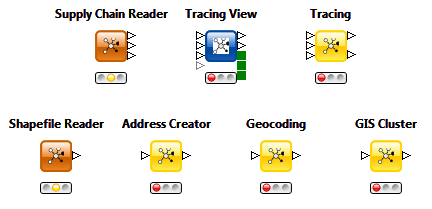
\includegraphics[height=0.4\textheight]{1.png}
	\end{center}
	\begin{itemize}
		\item Detailed descriptions of all nodes are available in the \textbf{Node Description} view of the KNIME workbench (\url{https://tech.knime.org/workbench}).
		\item All inputs and outputs are either \textbf{data tables} (triangles) or \textbf{images} (green square). Therefore standard KNIME nodes (\textbf{Row Filter}, \textbf{Image Port Writer}, ...) can be used in FoodChain-Lab workflows.		
	\end{itemize}
\end{frame}
 
\section{Tracing}
\begin{frame}
	\begin{center}
  		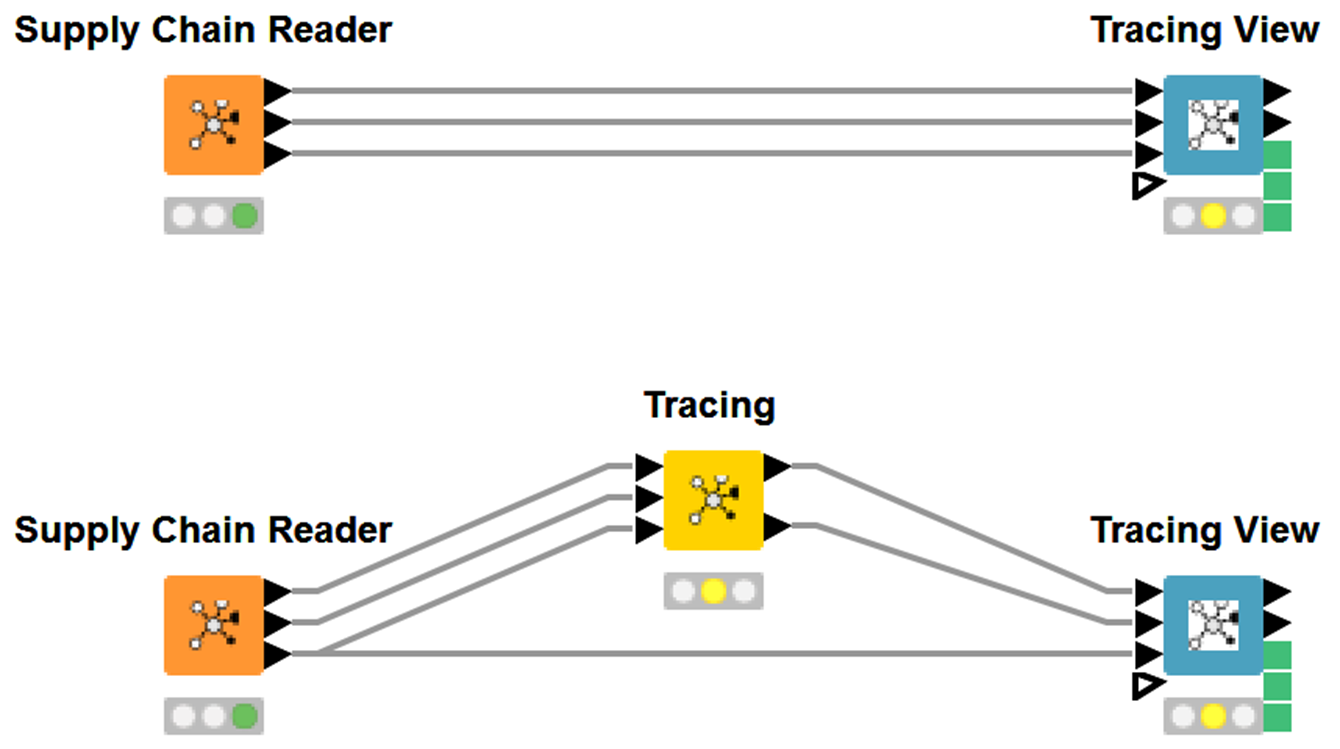
\includegraphics[height=0.4\textheight]{2.png}
	\end{center}
	\begin{itemize}
		\item Supply chain data is read from the internal database via the \textbf{Supply Chain Reader}.
		\item This data can be visualized with the \textbf{Tracing View}. The \textbf{Tracing View} also allows to perform a tracing on the data.
		\item The \textbf{Tracing} node performs tracing without visualization. Its output can be used in the \textbf{Tracing View} (e.g. to perform some tracings as a preprocessing step)
	\end{itemize}
\end{frame}

\section{Using GIS data}
\begin{frame}
	\begin{center}
  		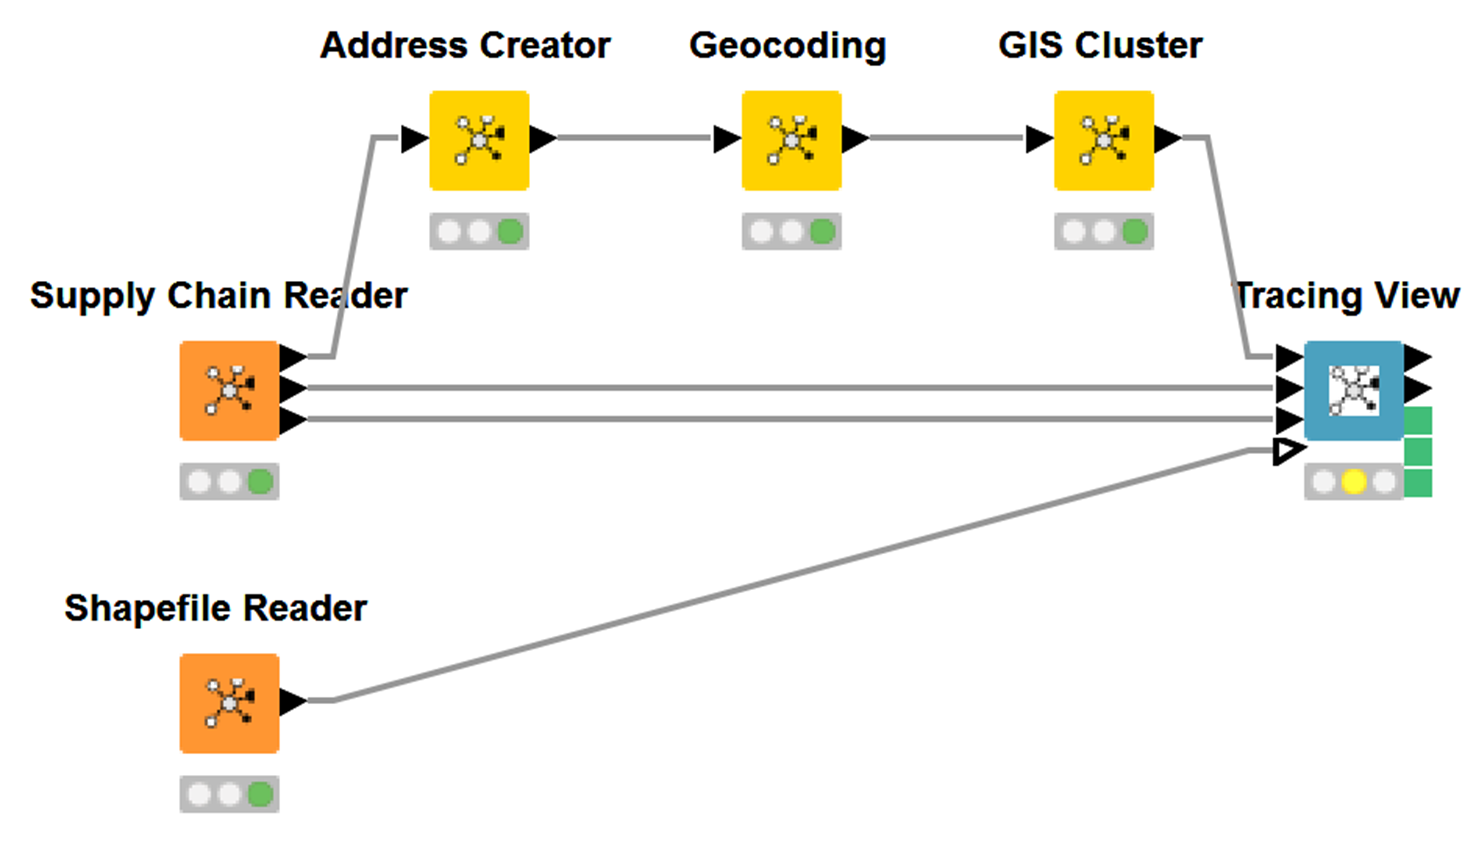
\includegraphics[height=0.6\textheight]{3.png}
	\end{center}
	\begin{itemize}
		\item The \textbf{Geocoding} node allows to acquire latitude/longitude data from addresses.
		\item This data can be geographically clustered with the \textbf{GIS Cluster} node.
		\item The \textbf{Tracing View} allows geographical visualization, if GIS data is provided from the \textbf{Shapefile Reader}.
	\end{itemize}		
\end{frame}

\end{document}